\chapter{Anexo}\label{ch:anexos}

\section{Gestión del proyecto}\label{sec:gestion-pr}

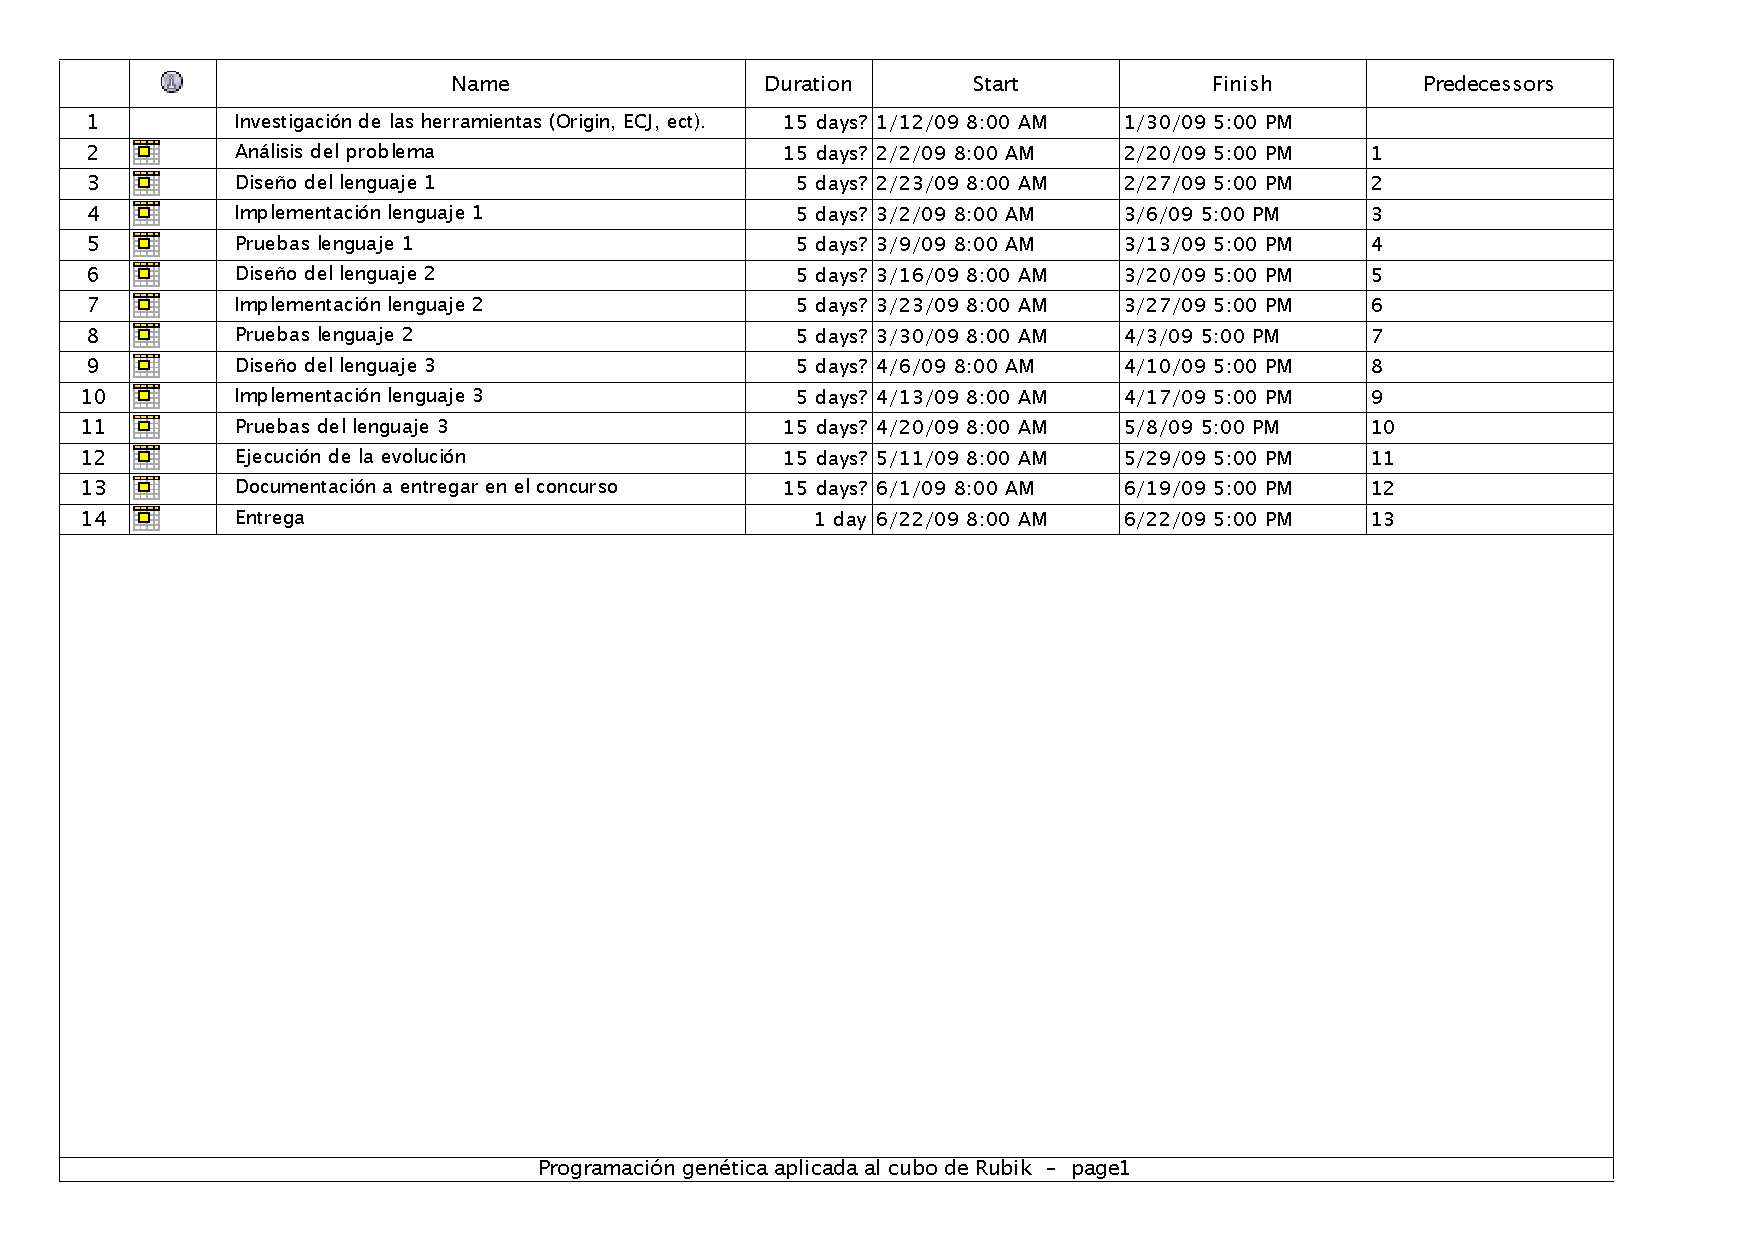
\includepdf[pages={1,2},landscape]{figs/planning.pdf}

\section{Parámetros de ECJ}\label{sec:ecj-params}

Fichero ec.params:

\begin{itemize}
\item verbosity = 0 : Es el nivel de mensajes que el sistema sacará por pantalla. Un número alto imprimirá más mensajes por pantalla.
\item	evalthreads=1 : Número de threads en el proceso de evaluación.
\item	breedthreads=1 : Número de threads en el proceso de reproducción.
\item	checkpoint=false : Activa o desactiva la opción de guardar el estado de
la evolución en una generación concreta.
\item	checkpoint-modulo = 1: Cada cuantas generaciones se haría el checkpoint.
\item	prefix = ec : Es el prefijo del nombre del fichero de checkpoint. 
\end{itemize}

El siguiente fichero en la jerarquía es simple.params. 

\begin{itemize}
\item	state = ec.simple.SimpleEvolutionState : esta clase define un modelo evolutivo generacional, es decir, cada generación es una nueva generación. Además se almacena la población de cada generación. Para poblaciones muy grandes y largas ejecuciones es mejor utilizar la clase  ec.steadystate.SteadyStateEvolutionState que mantiene una población, donde sus miembros van siendo reemplazados por los nuevos.
\item	init = 	ec.simple.SimpleInitializer : es la clase que se utilizará para inicializar la población.
\item	finish = ec.simple.SimpleFinisher :  es la clase que usa para finalizar
la población. Esta clase no hace nada actualmente.
\item	exch = ec.simple.SimpleExchanger : esta clase sirve para definir la forma
de intercambiarse individuos entre dos poblaciones. Esta clase tampoco hace nada.
\item	breed = ec.simple.SimpleBreeder : es la clase que asienta las bases de la reproducción. Se encargará de hacer el elitismo si se requiere. Sin embargo, esta clase solo escoge individuos dentro de la misma población.
\item	eval =	ec.simple.SimpleEvaluator :  es la clase que se encarga de administrar el procesos de evaluación de la población.
\item	stat =	ec.simple.SimpleStatistics : realiza estadísticas simples de la población.
\item	generations = 51 : número máximo de generaciones que podrán ejecutarse.
\item	quit-on-run-complete = true : activamos la opción de que el sistema pare cuando encontremos la mejor solución.
\item	pop = 	ec.Population : la clase de población que utilizaremos.
\item	pop.subpops = 1 : el número de subpoblaciones que tendremos
\item	pop.subpop.0 = ec.Subpopulation : la clase de subpoblación que existirá.
\item	pop.subpop.0.size =	1024 : el tamaño de la subpoblación 0
\item	pop.subpop.0.duplicate-retries = 0 : intentos de la subpoblación de eliminar los individuos repetidos de la población inicial 0.
\item	breed.elite.0 = 10 : espacio que dedicará para almacenar la élite de la población.
\item	stat.file \$out.stat : el nombre del fichero de estadísticas.
\end{itemize}

El próximo fichero en la jerarquía es koza.params:

\begin{itemize}
\item	pop.subpop.0.species.fitness = ec.gp.koza.KozaFitness : utilizaremos el fitness de koza.
\item	init = ec.gp.GPInitializer : Para inicializar la población se usará el inicializador de programación genética (GP).
\item	stat = ec.gp.koza.KozaStatistics : estadísticas de koza.
\item	pop.subpop.0.species = ec.gp.GPSpecies : especies de programación genética
\item	pop.subpop.0.species.ind = ec.gp.GPIndividual : individuos de programación genética.
\item	pop.subpop.0.duplicate-retries = 100 : se intentará 100 veces borrar a los individuos duplicados en la generación 0.
\item	pop.subpop.0.species.ind.numtrees = 1 : cada individuo tendrá un árbol.
\item	pop.subpop.0.species.ind.tree.0 = ec.gp.GPTree : este árbol será del tipo GPTree
\item	pop.subpop.0.species.ind.tree.0.tc = tc0 : Además tendrá la gramática tc0 (tree constrains).
\item	pop.subpop.0.species.pipe = ec.breed.MultiBreedingPipeline : lo individuos se someterán en la reproducción a varios sistemas de reproducción.
\item	pop.subpop.0.species.pipe.generate-max = false : no se intentará generar el máximo número de hijos.
\item	pop.subpop.0.species.pipe.num-sources = 2 : Se utilizarán dos formas de reproducción.
\item	pop.subpop.0.species.pipe.source.0 = ec.gp.koza.CrossoverPipeline : la primera será crossover.
\item	pop.subpop.0.species.pipe.source.0.prob = 0.9 : Se escogerá con una probabilidad de 0.9.
\item	pop.subpop.0.species.pipe.source.1 = ec.breed.ReproductionPipeline : en la segunda se utilizará la clonación.
\item	pop.subpop.0.species.pipe.source.1.prob = 0.1: con probabilidad 0.1.
\item	breed.reproduce.source.0 = ec.select.TournamentSelection : para seleccionar a los candidatos de la clonación se utilizará la selección por torneo(antes explicada).
\item	gp.koza.xover.source.0 = ec.select.TournamentSelection : para el proceso de crossover, el padre se buscará por el método de selección por torneo.
\item	gp.koza.xover.source.1 = same : la madre por el mismo sistema.
\item	gp.koza.xover.ns.0 = ec.gp.koza.KozaNodeSelector : para seleccionar el nodo en el padre que se cambiará, se utilizará el sistema de koza.
\item	gp.koza.xover.ns.1 = same : para la madre se utilizará el mismo sistema.
\item	gp.koza.xover.maxdepth = 17 : la máxima profundidad de los subárboles a escoger para el crossover será de 17 alturas.
\item	gp.koza.xover.tries = 1 : las veces que se intentará encontrar nodos compatibles para la reproducción.
\item	gp.koza.mutate.source.0 = ec.select.TournamentSelection : para mutar, se seleccionará a los individuos por torneo.
\item	gp.koza.mutate.ns.0 = ec.gp.koza.KozaNodeSelector : la selección del nodo a mutar se realizada por el método de Koza (aleatorio).
\item	gp.koza.mutate.build.0 = ec.gp.koza.GrowBuilder : Una vez que se localice el nodo, se reconstruirá el árbol por el método grow.
\item	gp.koza.mutate.maxdepth = 17 : es la profundidad máxima del subárbol a escoger. 
\item	gp.koza.mutate.tries = 1 : las veces que se intentará realizar la mutación con éxito.
\item	select.tournament.size = 7 : el número de individuos que entran en torneo.
\item	gp.koza.grow.min-depth = 5 : número de nodos mínimo de árbol del método grow.
\item	gp.koza.grow.max-depth = 5 : número máximo de nodos del método grow.
\item	gp.koza.ns.terminals = 0.1 : parámetro del selector de nodos, el cual seleccionará con probabilidad 0.1 terminales.
\item	gp.koza.ns.nonterminals = 0.9 : parámetro del selector de nodos, el cual seleccionará con probabilidad 0.9 noterminales.
\item	gp.fs.size = 1 : las siglas fs se refieren a Function Set. Sólo vamos a tener un grupo de funciones.
\item	gp.fs.0 = ec.gp.GPFunctionSet : nuestro grupo de funciones será del tipo GPFunctionSet.
\item	gp.fs.0.name = f0 : el nombre del grupo de función será f0.
\item	gp.type.a.size = 1 : tendremos solamente un tipo básico. Estos tipos básicos sirven para crear gramáticas y especifican el tipo de devuelta de los nodos.
\item	gp.type.a.0.name = nil : el nombre de este tipo básico es nil.
\item	gp.type.s.size = 0 : no tendremos ningún tipo compuesto.
\item	gp.tc.size = 1 : el tamaño de restricciones del árbol es de 1.
\item	gp.tc.0 = ec.gp.GPTreeConstraints : la clase para controlar estas restricciones es GPTreeConstraints.
\item	gp.tc.0.name = tc0 : el nombre de la restricciones sintácticas del árbol. Este debe coincidir con el especificado en el parámetro pop.subpop.0.species.ind.tree.0.tc.
\item	gp.tc.0.fset = f0 : el nombre del grupo de funciones.
\item	gp.tc.0.returns = nil : el tipo de devuelta del nodo base del árbol.
\item	gp.tc.0.init = ec.gp.koza.HalfBuilder : Es el constructor inicial del árbol. Mezcla el método grow y el método full.
\item	gp.koza.half.min-depth = 2 : es la mínima profundidad de los árboles generados.
\item	gp.koza.half.max-depth = 6 : es la profundidad máxima del árbol.
\item	gp.koza.half.growp = 0.5 : es la probabilidad que utilizará el método grow frente al método full.
\item	gp.nc.size = 7 : es el  número de restricciones sintácticas.
\item	gp.nc.0 = ec.gp.GPNodeConstraints : la clase que soporta estas restricciones.
\item	gp.nc.0.name = nc0 : el nombre de esta restricción.
\item	gp.nc.0.returns = nil : el tipo de devuelta esta restricción.
\item	gp.nc.0.size = 0 : el número de hijos que tendrá el nodo al que se aplique esta restricción. 
\item	gp.nc.1.child.0 = nil : cuando el número de hijos es mayor que cero hay que especificar el tipo de hijo que se requiere.
\end{itemize}

\section{Mejor Individuo}\label{sec:mejor-individuo}

(Progn2 (If (No (And (Test X1 Y1 FaceRight Color2) (Test X1 Y2 FaceBack Color1)))
(Move FaceDown Clockwise)) (Progn2 (If (No (And (Test X1 Y2 FaceUp Color1) (Test
X1 Y1 FaceFront Color5))) (Move FaceUp CounterClockwise)) (If (Or (Or (No (Test
X0 Y2 FaceUp Color1)) (Or (No (Test X0 Y2 FaceUp Color1)) (And (Test X1 Y1
FaceFront Color5) (And (No (And (Test X1 Y2 FaceUp Color1) (Test X1 Y1 FaceFront
Color5))) (Test X2 Y2 FaceFront Color1))))) (Or (Or (No (Test X0 Y2 FaceUp
Color1)) (And (And (And (Or (Or (No (Test X0 Y2 FaceUp Color1)) (Or (No (Test X0
Y1 FaceDown Color2)) (Test X0 Y2 FaceUp Color1))) (No (Or (Test X1 Y2 FaceUp
Color1) (Test X1 Y1 FaceDown Color2)))) (And (And (Test X1 Y1 FaceUp Color1)
(Test X1 Y1 FaceFront Color5)) (Or (No (Test X0 Y2 FaceUp Color1)) (And (And (And
(Test X1 Y1 FaceDown Color2) (Test X0 Y1 FaceDown Color2)) (Test X1 Y2 FaceUp
Color1)) (No (And (Test X1 Y1 FaceRight Color2) (Test X1 Y2 FaceBack
Color1))))))) (Test X1 Y2 FaceBack Color1)) (No (Test X2 Y2 FaceDown Color3))))
(No (Or (Or (Or (Or (Test X1 Y2 FaceUp Color1) (No (Test X1 Y2 FaceLeft Color0)))
(Test X1 Y1 FaceDown Color2)) (Test X1 Y2 FaceBack Color1)) (Test X1 Y1 FaceDown
Color2))))) (Move FaceLeft CounterClockwise))))
